This Chapter summarises the structure of the information necessary to define
the different input data to be used with the OpenQuake-engine risk 
calculators.

Input data for scenario-based and probabilistic seismic damage and risk
analysis using OpenQuake-engine are organised into:

\begin{itemize}

  \item A general calculation configuration file.

  \item A file describing the exposure model.

  \item A file describing the vulnerability model for loss calculations, or a 
  		file describing the fragility model for damage calculations. Optionally, 
  		a file describing the consequence model can also be provided in order 
  		to calculate losses from the estimated damage distributions.

  \item Hazard inputs

\end{itemize}

% Figure~\ref{fig:risk_input} summarises the structure of a risk input model
% for the OpenQuake-engine and the relationships between the different files.

% \begin{figure}[!ht]
% \centering
% \includegraphics[width=14cm]{figures/risk/risk_input_structure.pdf}
% \caption{PSHA Input Model structure}
% \label{fig:risk_input}
% \end{figure}

% \section{Defining Logic Trees}
% The main components of a logic tree structure in the OpenQuake engine are 
the following:
\begin{description}
    \item[branch]: the simplest component of a logic tree structure. 
    A branch represents a possible interpretation/value assignment of 
    a type of uncertainty. It is fully described by the tuple 
    (parameter/model, weight).
    
    \item[branching set]: a key component in the logic tree structure 
    used by the \gls{acr:oqe}. It groups a set of branches i.e. 
    alternative interpretations of a parameter or a model. Each branching
    set is defined by:
    \begin{itemize}
        \item An ID 
        \item An uncertainty type (for a comprehensive list of the types of 
        uncertainty currently supported see Section )
        \item One or more branches
    \end{itemize}
    
    This set of uncertainties can be applied to the whole initial 
    seismic source input model or just to a subset of seismic source
    data. The sum of the weights/probabilities assigned to the set 
    of branches. 

    \item[branching level]: the largest container. It's not used in 
    modelling uncertainty, but it's useful in maintaining a logic and an 
    order in the structure of the tree.
\end{description}

Below we provide a simple schema illustrating the skeleton of the 
\gls{acr:oqe} logic tree:
\begin{Verbatim}[frame=single, commandchars=\\\{\}, fontsize=\small]
\textcolor{green}{<logicTreeBranchingLevel branchingLevelID=ID>}
    \textcolor{blue}{<logicTreeBranchSet branchSetID=ID}
            \textcolor{blue}{uncertaintyType=TYPE>}
        \textcolor{magenta}{<logicTreeBranch>}
            \textcolor{cyan}{<uncertaintyModel>VALUE</uncertaintyModel>}
            \textcolor{cyan}{<uncertaintyWeight>WEIGHT</uncertaintyWeight>}
        \textcolor{magenta}{</logicTreeBranch>}
    \textcolor{blue}{</logicTreeBranchSet>}
\textcolor{green}{</logicTreeBranchingLevel>}
\end{Verbatim}

A schematic representation of these three objects is provided in Figure 
\ref{glts}. A branching level identifies the position in a tree where
branching occurs while a branch set identifies a collection of branches 
(i.e. individual branches) whose weights sum to 1.\\
%
\begin{figure}[!h]
\centering
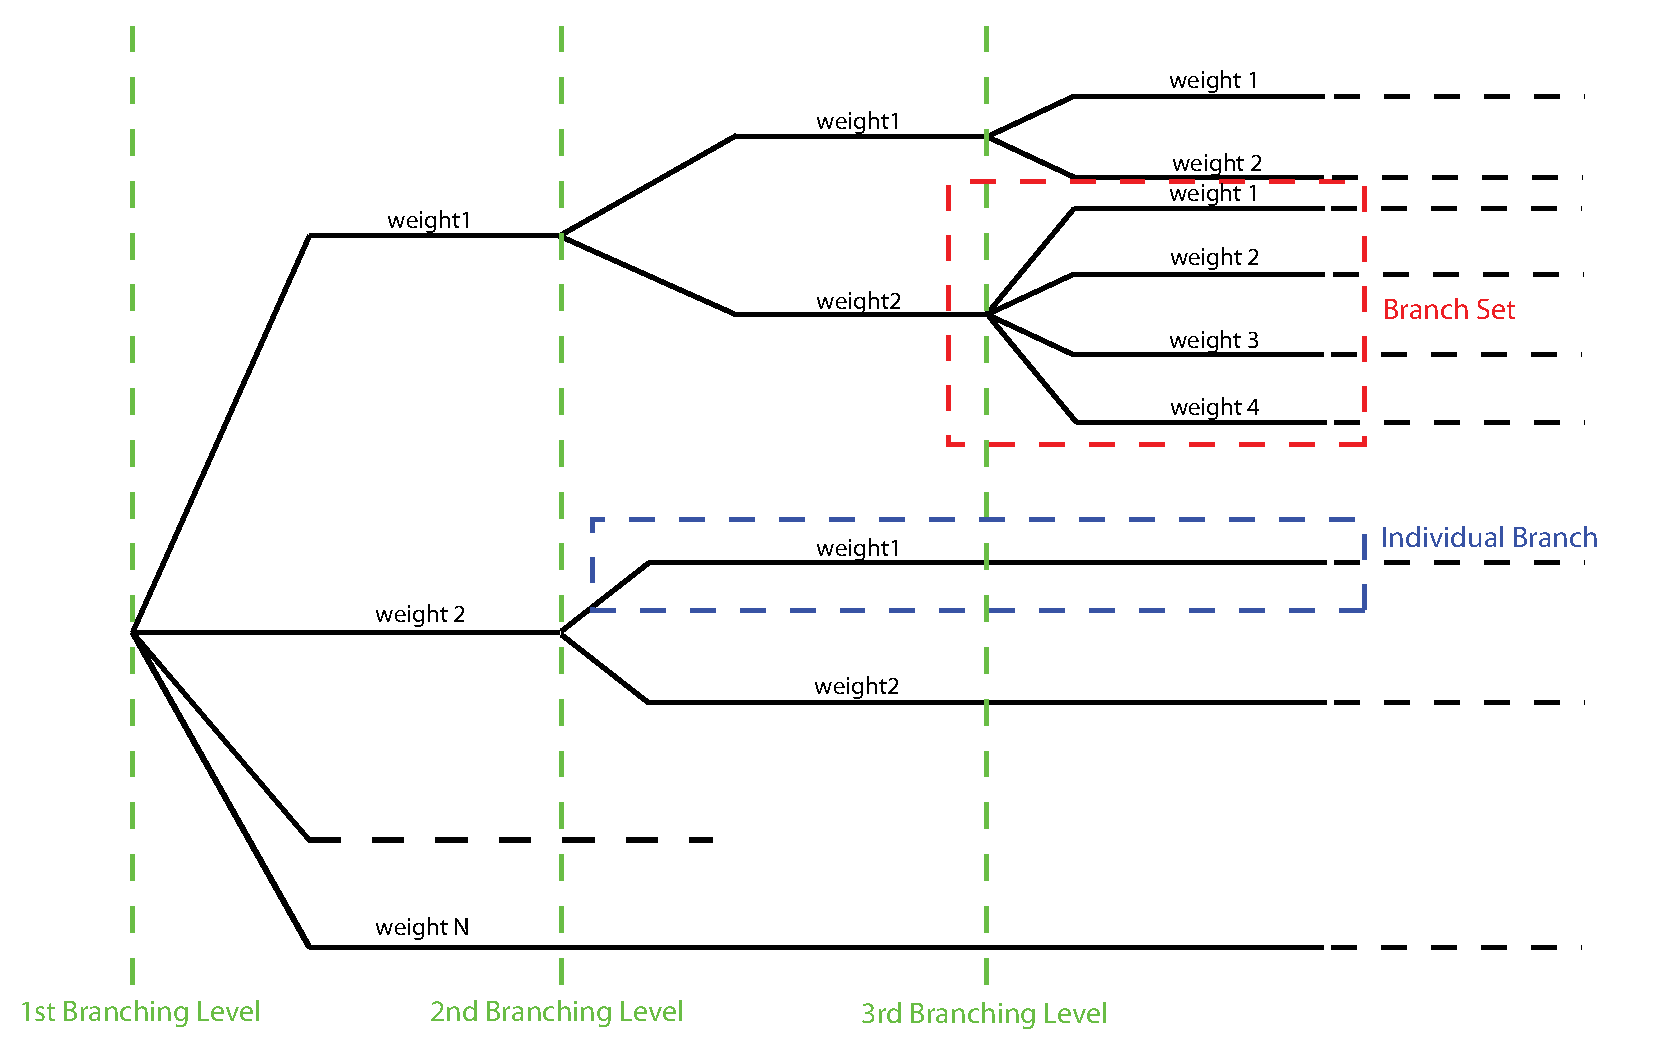
\includegraphics[width=15cm]{./figures/hazard/GenericLogicTreeStructure.eps}
\caption{Generic Logic Tree structure as described in terms of branching 
levels, branch sets, and individual branches.}
\label{glts}
\end{figure}
%
In the NRML schema, a logic tree structure is defined through the 
\Verb+logicTree+ element: 
%
\begin{Verbatim}[frame=single, commandchars=\\\{\}]
<\textcolor{red}{logicTree} logicTreeID="ID">
...
</\textcolor{red}{logicTree}>
\end{Verbatim}
%
A \Verb+logicTree+ contains as a sequence of \Verb+logicTreeBranchingLevel+ 
elements. The position in the sequence specifies in which level of the tree 
the branching level is located. That is, the first 
\texttt{logicTreeBranchingLevel} element in the sequence represents the first 
level in the tree, the second element the second level in the tree, and so on.
%
\begin{Verbatim}[frame=single, commandchars=\\\{\}]
<\textcolor{red}{logicTree} logicTreeID="ID">
	<\textcolor{green}{logicTreeBranchingLevel} branchingLevelID="ID_1">
		...
	</\textcolor{green}{logicTreeBranchingLevel}>
	<\textcolor{green}{logicTreeBranchingLevel} branchingLevelID="ID_2">
		...
	</\textcolor{green}{logicTreeBranchingLevel}>
	....
	<\textcolor{green}{logicTreeBranchingLevel} branchingLevelID="ID_N">
		...
	</\textcolor{green}{logicTreeBranchingLevel}>
</\textcolor{red}{logicTree}>
\end{Verbatim}
No restrictions are present on the number of tree levels that can 
be defined.

A \Verb+logicTreeBranchingLevel+ is defined as a sequence of 
\Verb+logicTreeBranchSet+ elements. Each \Verb+logicTreeBranchSet+ 
defines a particular epistemic uncertainty inside a branching level. 

A branch set has two required attributes (\Verb+branchSetID+ and 
\Verb+uncertaintyType+ (defining the type of epistemic uncertainty 
the branch set is defining))
\begin{Verbatim}[frame=single, commandchars=\\\{\}]
<\textcolor{red}{logicTree} logicTreeID="ID">
...
	<\textcolor{green}{logicTreeBranchingLevel} branchingLevelID="ID_#">
		<\textcolor{blue}{logicTreeBranchSet} branchSetID="ID_1"
			uncertaintyType="UNCERTAINTY_TYPE">
			...
		</\textcolor{blue}{logicTreeBranchSet}>
		<\textcolor{blue}{logicTreeBranchSet} branchSetID="ID_2"
			uncertaintyType="UNCERTAINTY_TYPE">
			...
		</\textcolor{blue}{logicTreeBranchSet}>
		...
		<\textcolor{blue}{logicTreeBranchSet} branchSetID="ID_N"
			uncertaintyType="UNCERTAINTY_TYPE">
			...
		</\textcolor{blue}{logicTreeBranchSet}>
	</\textcolor{green}{logicTreeBranchingLevel}>
...
</\textcolor{red}{logicTree}>
\end{Verbatim}
Possible values for the \Verb+uncertaintyType+ attribute are:
\begin{itemize}
\item \Verb+gmpeModel+: identifying epistemic uncertainties on ground 
motion prediction equations
\item \Verb+sourceModel+: identifying epistemic uncertainties on source models
\item \Verb+maxMagGRRelative+: identifying epistemic uncertainties 
(relative: that is increments) to be added (or subtracted, depending on 
the sign of the increment) to the 
Guten\-berg-Richter maximum magnitude value.
\item \Verb+bGRRelative+: identifying epistemic uncertainties (relative)
to be applied to the Guten\-berg-Richter b value.
\item \Verb+abGRAbsolute+:identifying epistemic uncertainties (absolute: 
that is new values used to replace original values) on the Guten\-berg-Richter
a and b values.
\item \Verb+maxMagGRAbsolute+: identifying epistemic uncertainties 
(absolute) on the Guten\-berg-Richter maximum magnitude.
\end{itemize}
No restrictions are given on the number of branch sets that can be defined 
inside a branching level.

A \Verb+branchSet+ is defined as a sequence of \Verb+logicTreeBranch+ 
elements, each specified by an \Verb+uncertaintyModel+ element (a string 
identifying an uncertainty mod\-el; the content of the string varies with
the uncertaintyType attribute value of the branchSet element) and the
uncertaintyWeight element (specifying the probability/weight associated 
to the uncertaintyModel):
\begin{Verbatim}[frame=single, commandchars=\\\{\}]
<\textcolor{red}{logicTree} logicTreeID="ID">
...
	<\textcolor{green}{logicTreeBranchingLevel} branchingLevelID="ID_#">
		...
		<\textcolor{blue}{logicTreeBranchSet} branchSetID="ID_#"
				uncertaintyType="UNCERTAINTY_TYPE">
			<\textcolor{magenta}{logicTreeBranch} branchID="ID_1">
				<uncertaintyModel>
				UNCERTAINTY_MODEL
				</uncertaintyModel>
				<uncertaintyWeight>
				UNCERTAINTY_WEIGHT
				</uncertaintyWeight>
			</\textcolor{magenta}{logicTreeBranch}>
			...
			<\textcolor{magenta}{logicTreeBranch} branchID="ID_N">
				<uncertaintyModel>
				UNCERTAINTY_MODEL
				</uncertaintyModel>
				<uncertaintyWeight>
				UNCERTAINTY_WEIGHT
				</uncertaintyWeight>
			</\textcolor{magenta}{logicTreeBranch}>
		</\textcolor{blue}{logicTreeBranchSet}>
		...
	</\textcolor{green}{logicTreeBranchingLevel}>
...
</\textcolor{red}{logicTree}>
\end{Verbatim}
Depending on the \Verb+uncertaintyType+ the content of the 
\Verb+<uncertaintyModel>+ element changes:
\begin{itemize}
\item if \Verb+uncertaintyType="gmpeModel"+, the uncertainty model 
contains the name of a ground motion prediction equation (a list of 
available GMPEs are given in appendix A), e.g.:
\begin{Verbatim}[frame=single, commandchars=\\\{\}]
<uncertaintyModel>GMPE_NAME</uncertaintyModel>
\end{Verbatim}
\item if \Verb+uncertaintyType="sourceModel"+, the uncertainty model contains 
the paths to a source model file, e.g.:
\begin{Verbatim}[frame=single, commandchars=\\\{\}]
<uncertaintyModel>SOURCE_MODEL_FILE_PATH</uncertaintyModel>
\end{Verbatim}
\item if \Verb+uncertaintyType="maxMagGRRelative"+, the uncertainty model 
contains the increment to be added (or subtracted, depending on the sign) 
to the Guten\-berg-Richter maximum magnitude:
\begin{Verbatim}[frame=single, commandchars=\\\{\}, samepage=true]
<uncertaintyModel>MAX_MAGNITUDE_INCREMENT</uncertaintyModel>
\end{Verbatim}
\item if \Verb+uncertaintyType="bGRRelative"+, the uncertainty model 
contains the increment to be added (or subtracted, depending on the 
sign) to the Guten\-berg-Richter b value:
\begin{Verbatim}[frame=single, commandchars=\\\{\}, samepage=true]
<uncertaintyModel>B_VALUE_INCREMENT</uncertaintyModel>
\end{Verbatim}
\item if \Verb+uncertaintyType="abGRAbsolute"+, the uncertainty model 
contains one (if the uncertainty apply to a source with only one 
Guten\-berg-Richter magnitude frequency distribution) or more (if the 
source has more than one magnitude frequency distributions) a and b pairs:
\begin{Verbatim}[frame=single, commandchars=\\\{\}, samepage=true]
<uncertaintyModel>
A_VALUE_1 B_VALUE_1
 ... 
A_VALUE_N B_VALUE_N
</uncertaintyModel>
\end{Verbatim}
    \item if \Verb+uncertaintyType="maxMagGRAbsolute"+, the uncertainty 
    model contains one or more (depending on the number of magnitude 
    frequency distributions in the source) Guten\-berg-Richter maximum 
    magnitude values:
%
\begin{Verbatim}[frame=single, commandchars=\\\{\}, samepage=true]
<uncertaintyModel>
MAX_MAGNITUDE_1
 ... 
MAX_MAGNITUDE_N
</uncertaintyModel>
\end{Verbatim}
\end{itemize}
%
No restrictions are given on the number of \Verb+logicTreeBranch+ elements 
that can be defined in a \Verb+logicTreeBranchSet+, as long as the uncertainty 
weights sum to 1.0.

The \Verb+logicTreeBranchSet+ element offers also a number of optional 
attributes allowing for complex tree definitions:
\begin{itemize}
    \item \Verb+applyToBranches+: specifies to which \Verb+logicTreeBranch+ 
    elements (one or more), in the previous branching level, the branch set 
    is linked to. The linking is established by defining the IDs of the 
    branches to link to:
\begin{Verbatim}[frame=single, commandchars=\\\{\}, samepage=true]
applyToBranches="branchID1 branchID2 .... branchIDN"
\end{Verbatim}
    The default is the keyword ALL, which means that a branch set is by default 
    linked to all branches in the previous branching level. By specifying one or 
    more branches to which the branch set links to, non-symmetric logic trees 
    can be defined.
    \item \Verb+applyToSources+: specifies to which source in a source model 
        the uncertainty applies to. Sources are specified in terms of their IDs:
\begin{Verbatim}[frame=single, commandchars=\\\{\}, samepage=true]
applyToSources="srcID1 srcID2 .... srcIDN"
\end{Verbatim}
    \item \Verb+applyToSourceType+: specifies to which source type the 
    uncertainty applies to.  Only one source typology can be defined 
    (\Verb+area+, \Verb+point+, \texttt{simple\-Fault}, 
	\Verb+complexFault+), e.g.:
\begin{Verbatim}[frame=single, commandchars=\\\{\}, samepage=true]
applyToSources="area"
\end{Verbatim}
    \item \Verb+applyToTectonicRegionType+: specifies to which tectonic 
    region type the uncertainty applies to. Only one tectonic region type 
    can be defined (\texttt{Ac\-tive} \texttt{Shallow Crust}, 
    \Verb+Stable Shallow Crust+, \Verb+Subduction Interface+, 
    \texttt{Sub\-duc\-tion} \texttt{IntraSlab}, \texttt{Volcanic}), e.g.:
\begin{Verbatim}[frame=single, commandchars=\\\{\}]
applyToTectonicRegionType="Active Shallow Crust"
\end{Verbatim}
\end{itemize}

% \label{sec:risk_logic_trees}

\section{Configuration file}
\index{Input!Configuration file}
\label{sec:risk_configuration_file}
The configuration file (or job.ini file) represents the location where the
paths to the input files, the parameters controlling the risk calculations and
the type of outputs are defined. Some initial parameters common to all the
risk calculators are presented below. The remaining parameters that are
specific to each risk calculator are discussed in subsequent sections. For
additional information about how each parameter is being used within the
methodologies implemented in the oq-engine, users advised to consult the
OpenQuake-engine Book (Risk).

\begin{Verbatim}[frame=single, commandchars=\\\{\}, samepage=true]
[general]
description = Scenario Risk Nepal
calculation_mode = scenario_risk

exposure_file = exposure_model.xml
region_constraint = 78.0 31.5,89.5 31.5,89.5 25.5,78 25.5
asset_hazard_distance = 10
...
\end{Verbatim}

\begin{itemize}
\item  \Verb+description+: a parameter that can be used to include some information about the type of calculations that are going to be performed;
\item  \Verb+calculation_mode+: this parameter sets the type of calculations. The key word for each risk calculator is described in the following sections;
\item  \Verb+exposure_file+: this parameter is used to specify the path to the \gls{exposure model} file;
\item  \Verb+region_constraint+: this field is used to define the polygon enclosing the region of interest. Assets outside of this region will not be considered in the risk calculations. This region is defined using pairs of coordinates (longitude and latitude in decimal degrees) that indicate the vertices of the polygon;
\item  \Verb+asset_hazard_distance+: this parameter indicates the maximum allowable distance between an \gls{asset} and the closest hazard input. If no hazard input is found within this distance, the \gls{asset} is skipped and a message is provided mentioning the id of the asset that is affected by this issue. If this parameter is not provided, the OpenQuake-Engine assumes the maximum allowable distance as 5 km.
\end{itemize}

Depending on the type of calculations, other parameters besides the
aforementioned ones need to be provided, as will be described in the following
sections.

\subsection{Scenario Damage Calculator}
\label{subsec:config_scenario_damage}
For this calculator, the parameter \Verb+calculation_mode+ needs to be defined as \Verb+scenario_damage+. There is only one parameter specific to this calculator, which is the \gls{fragility model} file path, as presented below.

\begin{Verbatim}[frame=single, commandchars=\\\{\}, samepage=true]
...
fragility_file = fragility_model.xml
\end{Verbatim}

\begin{itemize}
\item  \Verb+fragility_file+: a parameter used to define the path to the \gls{fragility model} file.
\end{itemize}

\subsection{Scenario Risk Calculator}
\label{subsec:config_scenario_risk}
In order to run this calculator, the parameter \Verb+calculation_mode+ needs to be set to \Verb+scenario_risk+. The remaining parameters are illustrated bellow.

\begin{Verbatim}[frame=single, commandchars=\\\{\}, samepage=true]
...
structural_vulnerability_file = struct_vul_model.xml
nonstructural_vulnerability_file = nonstruct_vul_model.xml
contents_vulnerability_file = cont_vul_model.xml
business_interruption_vulnerability_file = bus_int_vul_model.xml
occupants_vulnerability_file = occ_vul_model.xml

asset_correlation = 0.7
master_seed = 3
insured_losses = true
\end{Verbatim}

\begin{itemize}
\item  \Verb+structural_vulnerability_file+: this parameter is used to specify the path to the structural \gls{vulnerability model} file;
\item  \Verb+nonstructural_vulnerability_file+: this parameter is used to specify the path to the non-structural\gls{vulnerability model} file;
\item  \Verb+contents_vulnerability_file +: this parameter is used to specify the path to the contents \gls{vulnerability model} file;
\item  \Verb+business_interruption_vulnerability_file +: this parameter is used to specify the path to the business interruption \gls{vulnerability model} file;
\item  \Verb+vulnerability_file+: this parameter is used to specify the path to the occupants \gls{vulnerability model} file;
\item \texttt{asset\_cor\-re\-la\-tion} if the uncertainty in the loss ratios has been defined within the \gls{vulnerability model}, users can specify a coefficient of correlation that will be used in the Monte Carlo sampling process of the loss ratios, between the assets that share the same \gls{taxonomy}. If the \texttt{asset\_cor\-re\-la\-tion} is set to one, the loss ratio residuals will be perfectly correlated. On the other hand, if this parameter is set to zero, the loss ratios will be sampled independently. Any value between zero and one will lead to increasing levels of correlation. If this parameter is not defined, the OpenQuake-engine assumes no correlation in the vulnerability;
\item  \Verb+master_seed+: this parameter is used to control the random generator in the loss ratio sampling process. This way, if the same \Verb+master_seed+ is defined at each calculation run, the same random loss ratios will be generated, thus allowing replicability of the results;
\item  \Verb+insured_losses+: this parameter is used to define if insured losses should be calculated (\Verb+true+) or not (\Verb+false+).
\end{itemize}

\subsection{Classical Probabilistic Seismic Damage Calculator}
\label{subsec:config_classical_damage}
In order to run this calculator, the parameter \Verb+calculation_mode+ needs to be set to \Verb+classical_damage+. Similar to the Scenario Damage calculator, there is only one parameter specific to this calculator, which is the \gls{fragility model} file path, as presented below.
\begin{Verbatim}[frame=single, commandchars=\\\{\}, samepage=true]
...
fragility_file = fragility_model.xml
\end{Verbatim}

\subsection{Classical Probabilistic Seismic Risk Calculator}
\label{subsec:config_classical_risk}
In order to run this calculator, the parameter \Verb+calculation_mode+ needs to be set to \Verb+classical_risk+. With this calculator it is also possible to extract loss maps, so the parameter \Verb+conditional_loss_poes+ needs to be defined as explained in the previous sub-section. The remaining parameters are illustrated below:
\begin{Verbatim}[frame=single, commandchars=\\\{\}, samepage=true]
...
structural_vulnerability_file = struct_vul_model.xml
nonstructural_vulnerability_file = nonstruct_vul_model.xml
contents_vulnerability_file = cont_vul_model.xml
business_interruption_vulnerability_file = bus_int_vul_model.xml
occupants_vulnerability_file = occ_vul_model.xml

lrem_steps_per_interval = 2
conditional_loss_poes = 0.01, 0.05, 0.10
\end{Verbatim}

\begin{itemize}
\item  \Verb+lrem_steps_per_interval+: this parameter controls the number of intermediate values between consecutive loss ratios (as defined in the \gls{vulnerability model}) that are considered in the risk calculations. A larger number of loss ratios than those defined in each \gls{vulnerability function} should be considered, in order to better account for the uncertainty in the loss ratio distribution. If this parameter is not defined in the configuration file, the OpenQuake-engine assumes the \Verb+lrem_steps_per_interval+ to be equal to 5. More details are provided in the OpenQuake-engine Book (Risk).
\end{itemize}

\subsection{Event-Based Probabilistic Seismic Risk Calculator}
\label{subsec:config_event_based_risk}
The parameter \Verb+calculation_mode+ needs to be set to \Verb+event_based_risk+ in order to use this calculator. Similarly to that described for the Scenario Risk Calculator, a Monte Carlo sampling process is also employed within this module to take into account the loss ratio uncertainty. Hence, the parameters \Verb+asset_correlation+ and \Verb+master_seed+ need to be defined as previously described. This calculator is also capable of estimating insured losses and therefore, the \Verb+insured_losses+ attribute should be specified as well. The parameter ``risk\_investigation\_time'' specifies the time period for which the event loss tables and loss exceedance curves will be calculated. If this parameter is not provided in the risk job configuration file, the time period used is the same as that specifed in the hazard calculation. The Probabilistic Event-based Risk Calculator can disaggregate the losses based on magnitude/distance and location (longitude/latitude) of the events. In order to do so, it is necessary to define the bin width of each of these parameters, as illustrated in the following example.

The remaining parameters are presented below.

\begin{Verbatim}[frame=single, commandchars=\\\{\}, samepage=true]
...
structural_vulnerability_file = struct_vul_model.xml
nonstructural_vulnerability_file = nonstruct_vul_model.xml
contents_vulnerability_file = cont_vul_model.xml
business_interruption_vulnerability_file = bus_int_vul_model.xml
occupants_vulnerability_file = occ_vul_model.xml

asset_correlation = 0.7
master_seed = 3
insured_losses = true

sites_disagg = 85.07917, 27.4625
mag_bin_width = 0.5
distance_bin_width = 20
coordinate_bin_width = 0.5

specific_assets = asset_11 asset_132 asset_303 asset_611

loss_curve_resolution = 20
conditional_loss_poes = 0.01, 0.05, 0.10
\end{Verbatim}

\begin{itemize}
\item \Verb+loss_curve_resolution+: since this calculator uses an event\--based ap\-proach, a large number of levels of loss (and associated probabilities of exceedance) is computed (one per event) for each asset. The oq-risklib will use this large set of results to extrapolate a loss curve, whose number of points are controlled by this parameter. By default, the OpenQuake-engine assumes the \Verb+loss_curve_resolution+ equal to 20;
\item  \Verb+risk_investigation_time+: this parameter specifies the time period for which the event loss tables and loss exceedance curves will be calculated. If this parameter is not provided in the risk job configuration file, the time period used is the same as that specifed in the hazard calculation;
\item  \Verb+conditional_loss_poes+: this parameter is used to define the probabilities of exceedance at which loss maps are to be produced;
\item  \Verb+sites_disagg+: list of locations (pairs of longitude and latitude) where the loss disaggregation should be carried out. Notice that in order to perform the loss disaggregation, assets needs to exist at those locations;
\item  \Verb+mag_bin_width+: this parameter specifies the with of the magnitude bins (in Mw);
\item  \Verb+distance_bin_width+: this parameter specifies the with of the distance bins (in km);
\item  \Verb+coordinate_bin_width+: this parameter specifies the with of the coordinates bins (in decimal degrees);
\item  \Verb+specific_assets+: this parameter specifies the set of assets for which the asset event loss table will be generated;
\end{itemize}

The definition of the parameters for the loss disaggregation follow the same rules established for the seismic hazard disaggregation described in section~\ref{subsec:config_hazard_disaggregation}.

\paragraph{Note regarding the new event-based risk calculators}

Starting from this release some of the scientific calculators are saving their inputs and outputs in a single HDF5 file, called the datastore. The HDF5 format is a well known standard in the scientific community, can be read/written by a variety of programming languages and with different tools and it is a state-of-the-art technology when it comes to managing large numeric datasets. The change to the HDF5 technology provides huge performance benefits compared to the earlier approach used by the engine, which involved storing arrays in PostgreSQL.

In OpenQuake 1.5 the event based calculators based on Postgres (both hazard and risk) are officially deprecated. They are still present and work as before, but they are being replaced with new versions of the calculators based on the HDF5 technology. The actual removal of the old calculators is scheduled for OpenQuake 1.6. The change will have no impact on regular users, who will simply notice a definite improvement in erformance. Nonetheless, the change will affect power users who are performing queries on the OpenQuake database, since there will be nothing left in the database once we remove the old calculators.

In order to make the transition easier, OpenQuake 1.5 already includes the new versions of the event based calculators based on HDF5, so it is possible to use them right now. The new calculators can be run in OpenQuake 1.5 with the command:

\begin{Verbatim}[frame=single, commandchars=\\\{\}, fontsize=\small]
user@ubuntu:~$ oq-engine --lite --run job_haz.ini,job_risk.ini
\end{Verbatim}

If you do not pass the --lite flag the old calculators will be run by default. In future releases of the engine, the remaining calculators based on Postgres will be progressively replaced by the new calculators based on HDF5. At the end of this process, which will be spread over several upcoming releases, the --lite flag will be removed. All of the old calculators relying on the database will be replaced internally by the newer ``lite'' versions based on HDF5 and the old calculators will not be available anymore. The OpenQuake database will only contain accessory information (essentially a table with the users and references to the outputs of each user) but nothing relevant for the scientific computation.

\subsection{Retrofit Benefit-Cost Ratio Calculator}
\label{subsec:config_benefit_cost}
As previously explained, this calculator uses loss exceedance curves which are calculated using the Classical PSHA-based Risk calculator. The \Verb+calculation_mode+ should be set to \Verb+classical_bcr+ and the calculator-specific part of the configuration file should be defined as presented below.

\begin{Verbatim}[frame=single, commandchars=\\\{\}, samepage=true]
...
structural_vulnerability_file = structural_vulnerability_model.xml
vulnerability_retrofitted_file = retrofitted_vulnerability_model.xml

lrem_steps_per_interval = 2

interest_rate = 0.05
asset_life_expectancy = 50
\end{Verbatim}

\begin{itemize}
\item  \Verb+vulnerability_retrofitted_file+: this parameter is used to specify the path to the \gls{vulnerability model} file containing the \glspl{vulnerability function} for the retrofitted assets;
\item  \Verb+interest_rate+: this parameter represents the interest rate and it serves the purposes of taking into account the variation of building value throughout time;
\item  \Verb+asset_life_expectancy+: this variable defines the life expectancy, or design life, of the assets.
\end{itemize}

\cleardoublepage